\chapter{Wave mechanics}
\section{Double-slit experiment}
Material for this chapter can be found in the book by Feynman and Hibbs. The experimental setup is outlined in Figure 1.1: a source emits particles (electrons, photons, ...) which impinge on a double-slit screen. The particles propagating through the two columns are registered with a suitable detector.
%图1.1
\begin{figure}[ht]
    \centering
    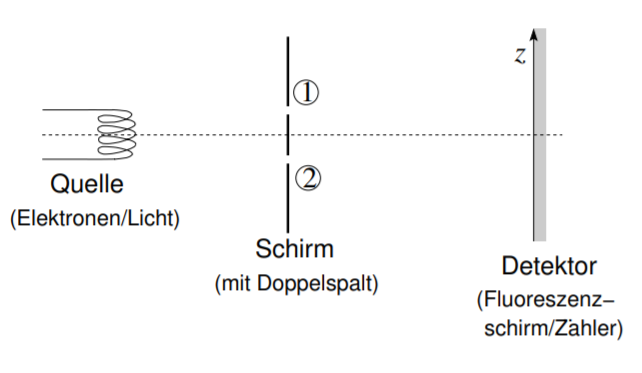
\includegraphics[scale=1]{1_1.PNG}
    \captionsetup{font={Large}}
    \caption{The double-slit experiment: those emitted by the source particles/waves hit a screen with two overlays columns and are analyzed in the detector.}
    \label{fig:1.1}
\end{figure}
\\
The result of the measurement is shown in Figure 1.2 where I = intensity, in $[I]$ = number of particles/s is measured. For a gap (without diffraction), the result for waves and particles looks the same according to classical expectation (see $I_1$ and $I_2$). If both slots are used, one expects (classical) different results, $I_w$ for waves and $I_k$ for particles. However, the experimental result of the double-slit experiment with particles again shows an interference pattern in the intensity, which leads to the conclusion
%PAGE 16
to draw is that the particles propagate like waves.
%图1.2
\begin{figure}[ht]
    \centering
    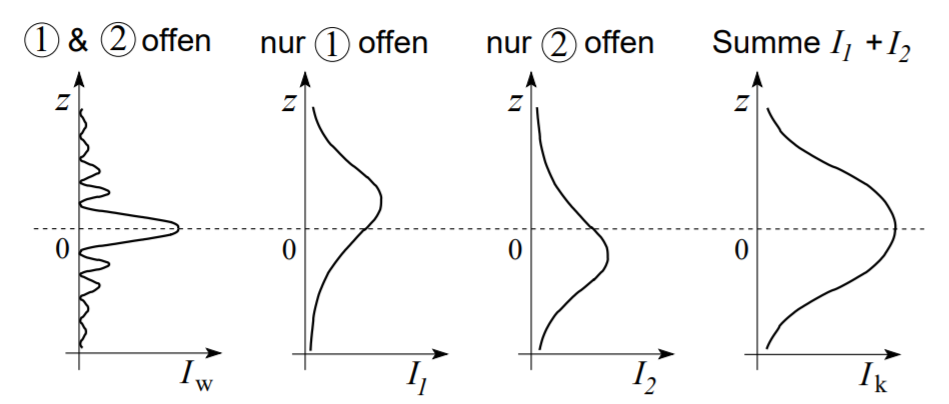
\includegraphics[scale=1]{1_2.PNG}
    \captionsetup{font={Large}}
    \caption{Left: the intensity at $I_w$ is the classically expected interference pattern for waves. The same result is found for the experiment with particles. Right: the intensity $I_k$ is the classically expected result for particles, but is not observed. The conclusion from the experiment is that particles propagate like waves.}
    \label{fig:1.2}
\end{figure}
Also with the detection one finds an unexpected result: becomes classical expected a discrete detection of particles. In contrast, one expects
classic for the intensity of waves a continuous result. The experiment also shows discrete events for the detection of waves, see. Figure  1.3.
%PAGE17
%图1.3
\begin{figure}[ht]
    \centering
    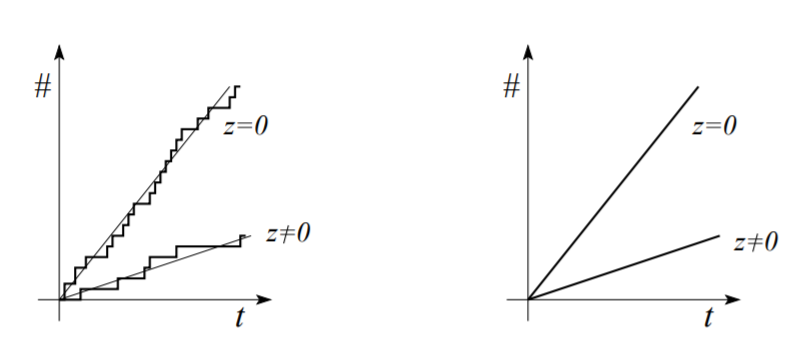
\includegraphics[scale=1]{1_3.PNG}
    \captionsetup{font={Large}}
    \caption{Left: Discrete detection is expected for classical particles. The same finding is obtained for the detection of waves. Right: Continuous detection is expected for waves but is not observed experimentally. One concludes that waves are detected like particles.}
    \label{fig:1.3}
\end{figure}
\\ \\
In summary, the following conclusions are drawn from the experimental findings:
%流程图
in the following we want to formalize this finding. Were we the double-slit experiment classically interpreted, the particle would either have to \ding{172} or \ding{173} happen. Let us denote $P_i(z), i = 1, 2$, as (relative) probability
%PAGE 18
for passage of particles through columns 1 or 2 and subsequent ones detection in $z$ would have been done in open \ding{172} and \ding{173} classical result
\\
\begin{equation}
P(z)=\sum_{i} P_{i}(z) \quad \text { (particle) }
\end{equation}
%公式1.1
expect. On the other hand, for waves we would have an amplitude $\Phi_i(z)$ kidney and the (relative) probability $w$ are then given by
$P_i(z)=| \Phi_i(z) |^2$ if only gap
\textcircled{i} is. If, on the other hand, the columns \ding{172} and \ding{173}, so one expects interference according to
\\
\begin{equation}
P(z)=\left|\sum_{i} \Phi_{i}(z)\right|^{2} \quad \text { (Wellen) }
\end{equation}\\
%公式1.2
The experiment gives the result that the particles are the same probability distribution $P (z)$ as the waves generate, therefore must it is also possible to assign a probability amplitude $\Phi_i (z) \in C$ to the particles and how waves demand the validity of the superposition principle. The problem now arises that one is under a particle, at least according to our perception, always presents a small body, but then either through the gap \ding{172} or \ding{173} the gap to the detector arrives. This contradiction motivates an extension of the experiment in that one measures by what gap the particle to detector arrives, see Figure  1.4.
%图1.4
\begin{figure}[ht]
    \centering
    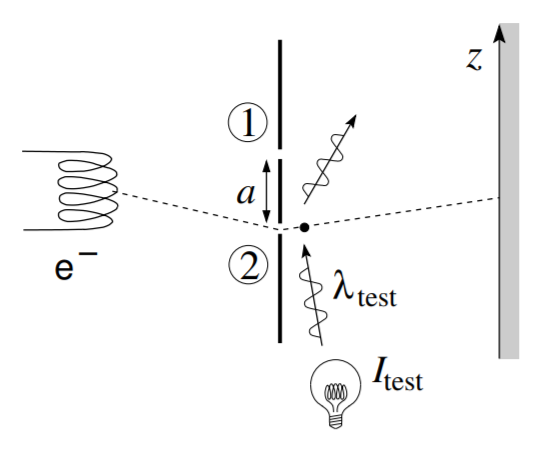
\includegraphics[scale=1]{1_4.PNG}
    \captionsetup{font={Large}}
    \caption{Double slit experiment with detection: Light emitted by the lamp should show the passage of the particle through the gap \ding{173}.}
    \label{fig:1.4}
\end{figure}
\\ \\So we're counting a particle, whenever it's through gap \ding{173}, that is, it must apply now that
\\
\begin{equation}
P=P_{1}+P_{2}
\end{equation}\\
%公式1.3
%PAGE19
is. In fact, this expectation agrees with the result of the experiment. Apparently there is a paradoxical situation here.\\
Next, we minimize the problem by testing with the lamp by reducing the intensity, $I_{test}\to 0$. Once $I_{test}$ is so small that Do not scatter the individual photons at each electron (see Comptoneekt) $P = P1 + P2$ in $P = | \Sigma_i \Phi_i|^2$ about. On the other hand, we can minimize the problem with the test by setting the wavelength of the test Light up, $\lambda_{test}\to \infty$(It does not matter whether we are actually interested in the measurement result or not, it's all about having the measurement results in principle by the lamp behind the double slit the passage of the particles is detected.). Once $\lambda_{test}$ is so large that the distance a is not can be solved more, $P = P1 + P2$ in $P = | \Sigma_i \Phi_i|^2$. If so at least in principle we know whether the particle is now via \ding{172} or \ding{173} to the detector we get $P = \Sigma_i P_i$ otherwise $P = | \Sigma_i \Phi_i|^2$.\\
An experiment that gives the information about the particle taken by the particle path returns (`which path detection'), so it locates the original experiment so strong that the interference is destroyed [see also E. Buks, R. Schuster, M. Heiblum, D. Malahu and V. Umansky, Nature 391, 871 (1998)]. This is a direct manifestation of Heisenberg's principle of blurring. This principle guarantees the consistency of the approach $P = | \Sigma_i \Phi_i|^2$ for propagation the particles; as long as the principle of blur applies, there is no paradox. Till today, all experiments are in harmony with the principle of blur. For a better understanding/proof we will consider a new experiment, whose structure is shown in Figure  1.5.\\
In experiment the spreader (here a screen with a double slit) becomes so set up an electron which passes through the gap \ding{172} i.e., a deflection $\delta z> 0$, one through the gap \ding{173}, a shift $\delta z <0$ is generated. Particles with momentum $p$ generate an interference pattern with $d$ given by ($p = h/ \lambda$, see Figure  1.5)
\\\begin{equation}
\frac{\lambda}{a} \sim \frac{d}{l}
\end{equation}
\\
%公式1.4
The momentum difference $\delta p_z = | p_z^{\ding{172}}$ for particles, which by \ding{172} or \ding{173}, is $\delta p_z \sim pa/l=h/d$. Let's see if choosing the way \ding{172} or \ding{173}, we have to reach an accuracy $\Delta p_z < \delta p_z$. But we want additionally to see the interference pattern, the position $z$ of the screen with be known to the gap up to $\Delta z <d$, since a larger deflection a `Smearing the maxima' entails. Do we want both results, see the information about the path and the interference realized, then $\Delta p_z \Delta z <h$ must be in contradiction to the principle of uncertainty.
%PAGE 20
%图1.5
\begin{figure}[ht]
    \centering
    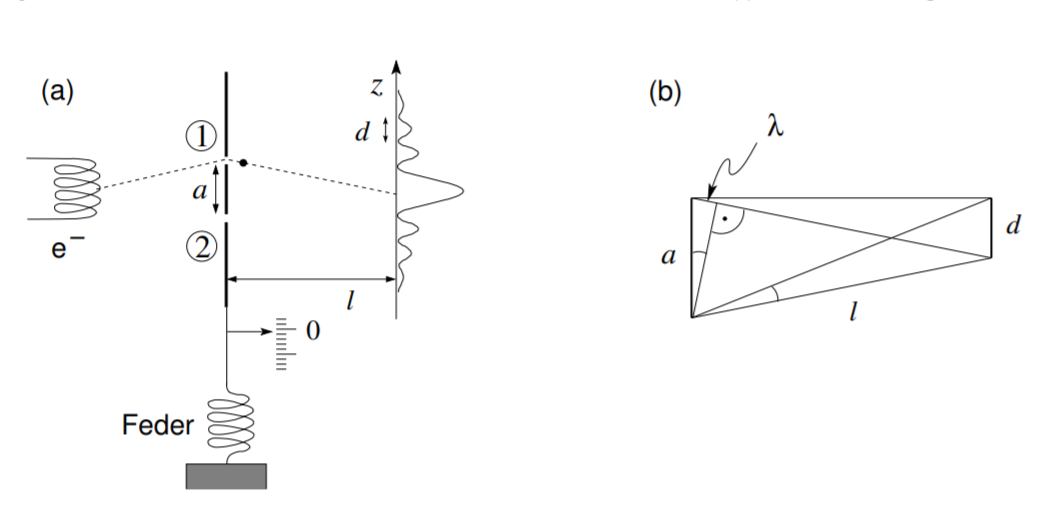
\includegraphics[scale=1]{1_5.PNG}
    \captionsetup{font={Large}}
    \caption{Double-slit experiment with detection: The deflection of the screen is intended to give indications of the passage of the small particle. This arrangement automatically leads to the Heisenberg uncertainty principle.}
    \label{fig:1.5}
\end{figure}
\\ \\
In summary, we note the following points:
\begin{itemize}
    \item[-] Propagation: Propagation always happens as a wave and involved the amplitude $\Phi$.
    \item[-] Detection: Detection always happens as particles and involved the probability $P = | \Phi |^2$.
    \item[-] Observation: Any observation fixes the propagation and destroys place the interference formation $\Phi = \sum_i \Phi_i$ in the total amplitude.
\end{itemize}

The consistency of QM demands even more astonishing effects: instead of the alternatives in the double-slit scattering experiment we consider the Figure 1.6 sketched particle-particle scattering with also two alternatives (here the so-called 'quantum alternatives' replace the simple paths).\\
Let $\Phi_{AB}(i, j)$ be the amplitude for the process (or quantum alternative) particle from A according to $i$, that of B according to $j$. From the symmetry of arrangement follows immediately: $\Phi_{AB}(1, 2) = \Phi_{AB}(2, 1)$. Are the particle types different in A and B, it is always possible to determine which type of particle in which detector arrived. There is no interference between the `paths' $A\to 1, B\to 2$ and $A\to 2, B\to 1$ and the coincidence measurement is by the probability
\begin{equation}
P_{\text {Koin }}=\left|\Phi_{\mathrm{AB}}(1,2)\right|^{2}+\left|\Phi_{\mathrm{AB}}(2,1)\right|^{2}=2 p
\end{equation}
%公式1.5
%图1.6
\begin{figure}[ht]
    \centering
    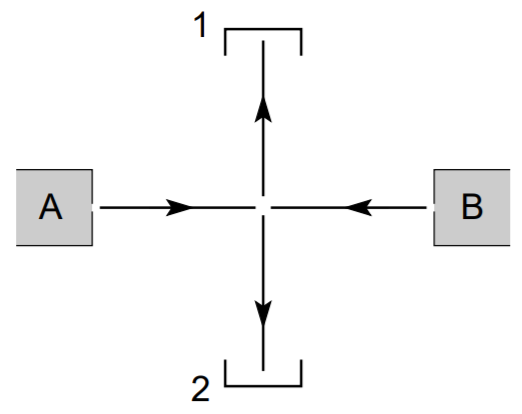
\includegraphics[scale=1]{1_6.PNG}
    \captionsetup{font={Large}}
    \caption{Particle Scattering: particles are emitted from sources A and B and measured in detectors 1 and 2.}
    \label{fig:1.6}
\end{figure}
%PAGE21
\\ \\
(PKoin gives the probability of having a particle in the same time to measure detector 1 and the second particle in Figure 2.) Are the particles identical,
about $^{4}He$, $\alpha$-particles, spin-0-bosons, so we can do the 'paths' do not differ and therefore get 
\\
\begin{equation}
P_{\mathrm{Koin}}=\left|\Phi_{\mathrm{AB}}(1,2)+\Phi_{\mathrm{AB}}(2,1)\right|^{2}=4 p
\end{equation}\\
%公式1.6
in accordance with the experiments. If you bring the experiment with your identical particles such as $^{3}He$ atoms, protons $p$, neutrons $n$, electrons $e^-$, or other so-called spin-1 = 2 fermions, so the paths are still indistinguishable (if the spins are aligned the same way), but we receive(if the spins are different, we get again $P_{Koin} = 2p$, since here is a criterion to distinguish the particles, the interference of both paths therefore
get lost.)
\\
\begin{equation}
P_{\mathrm{Koin}}=\left|\Phi_{\mathrm{AB}}(1,2)-\Phi_{\mathrm{AB}}(2,1)\right|^{2}=0
\end{equation}\\
%公式1.7
The result for bosons is in direct agreement with the conjecture
\\
$$
P_{\mathrm{Koin}}=\left|\sum_{\text {Pfade }} \Phi_{\mathrm{Pfad}} \mathrm{c}\right|^{2}
$$\\
%公式
we sum the amplitudes before squaring over paths C and generate thus an interference term. At Fermions you'll find exactly how bosons interfere with the same spins, however, the `swapped' paths $A\to 1, B\to 2$ and $A\to 2, B\to 1$ with different signs
into the sum,
\\
$$
P_{\mathrm{Koin}}=\left|\sum_{\text {Pfade }}(-1)^{v} \Phi_{\mathrm{Plad}} \mathrm{C}\right|^{2}
$$
$$
P_{\mathrm{Koin}}=\left|\sum_{\text {Pfade }}(-1)^{v} \Phi_{\mathrm{Plad}} \mathrm{C}\right|^{2}
$$\\
%公式
Another consistent input gives neutron scattering with polarized
%PAGE 22
%图1.7
\begin{figure}[ht]
    \centering
    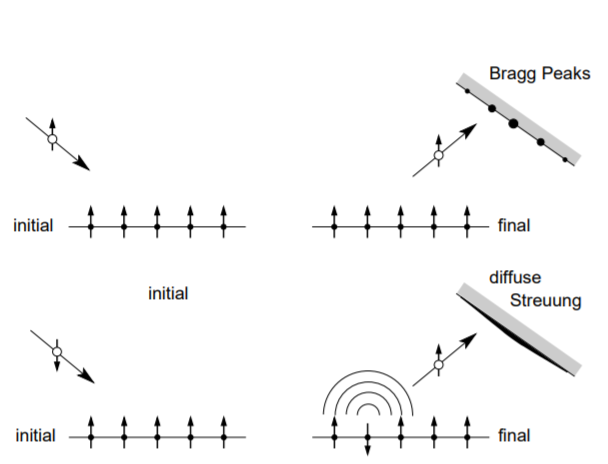
\includegraphics[scale=1]{1_7.PNG}
    \captionsetup{font={Large}}
    \caption{Scattering of neutrons on atoms with polarized spins. The interference is destroyed when the neutron releases a spin excitation that allows the scatter partner to identify itself.}
    \label{fig:1.7}
\end{figure}
neutrons on the polarized crystal, such as Figure 1.7: here two interference terms due to the summation over different scattering paths.
This interference is destroyed as soon as the information at which atom
neutron scattered was available. These experiments and ideas
lead us to a method for calculating the probabilities $P$
for a process: in order to find $P$ we have to use the possibly indistinguishable ones
determine and sum paths C and their amplitudes $\Phi_{PathC}$
according to (1.1).
For one-particle problems, $ v = 0$ and a path represents a path in the
physical space $\mathbb{R}^n$ represents; the probability for a process is
then through
\\
\begin{equation}
P=\left|\sum_{\text {Paths }} \Phi_{\text {Pfad }} C\right|^{2}
\end{equation}
%公式1.8
given. The two problems that need to be solved are:
\begin{itemize}
    \item What is the amplitude path $\Phi_{Pfad C}$ for any path $C$?
    \item Which means $\sum_{Paths}$?
\end{itemize}

\section{Path Integrals} 
There are usually not just two classical paths, but infinitely many paths,
see Figure 1.9.3(It puts a magnetic flux behind in an experiment with electrons the screen and between the paths (without the particles tracing a field)
this one additional phase diversity $(1/\Phi_0)\int Adl = \Phi/\Phi_0, \Phi_0=hc/e$ between the two paths which displace the interference pattern on the detector screen-- this is the famous Aharonov-Bohm Effect (1959), possibly discovered by Walter
Franz in Danzig (1939) and Werner Ehrenberg and Ray Siday (1949) in London, cf.
arXiv: 1304.4736v1.)
%PAGE 23
%图1.8 1.9
\begin{figure}[ht]
    \centering
    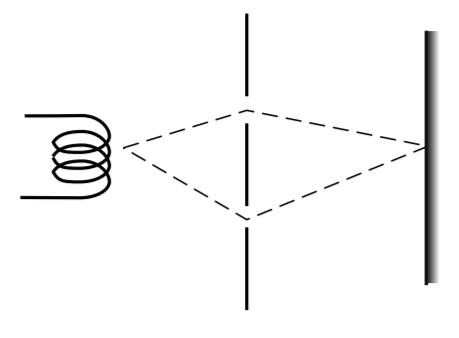
\includegraphics[scale=1]{1_8.PNG}
    \captionsetup{font={Large}}
    \caption{Two classic paths connect the source and
    the detector.}
    \label{fig:1.8}
\end{figure}
\begin{figure}[ht]
    \centering
    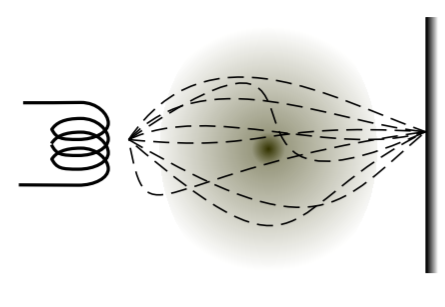
\includegraphics[scale=1]{1_9.PNG}
    \captionsetup{font={Large}}
    \caption{In quantum mechanics, all paths leading from the source to the detector contribute to the result.}
    \label{fig:1.9}
\end{figure}
\\ \\
A path is a function $y (x)$ or, in parametric form, a vector $(x (t), y (t))$ with the curve parameter $t$. Obviously, with $t$ mostly
meant the time. In general, a path is a vector-valued function $\vec{r} (t)$,
$\vec{r} \in \mathbb{R}^n$, where $\vec{r}$ indicates the position.

\subsection{Classical mechanics}
In classical mechanics, the movement of a particle realizes exactly one path $\vec{r} (t)$, namely, the one with the smallest effect. We consider the one-dimensional case. Let $L (x; \dot{x}; t)$ be the Lagrange function, $S=\int_{ta}^{tb}dtL(x,\dot{x}, t)$ the effect; their variation $\delta S = 0$ gives us the classical path $\bar{x}$ as a solution to an initial value problem. Explicit you are for the variation (use the functional derivative $\delta f (x)/\delta f(x') = \delta(x-x')$
in combination with the chain rule and a partial integration; here,
$f (x)\to x (t))$
\\
\begin{equation}
\begin{aligned} \frac{\delta \mathcal{S}\left[x\left(t^{\prime}\right)\right]}{\delta x(t)} &=\int_{t_{a}}^{t_{b}} d t^{\prime}\left[\frac{\partial \mathcal{L}}{\partial x} \frac{\delta x\left(t^{\prime}\right)}{\delta x(t)}+\frac{\partial \mathcal{L}}{\partial \dot{x}} \frac{\delta \dot{x}\left(t^{\prime}\right)}{\delta x(t)}\right] \\ &=\int_{t_{a}}^{t_{b}} d t^{\prime}\left[\frac{\partial \mathcal{L}}{\partial x} \delta\left(t-t^{\prime}\right)+\frac{\partial \mathcal{L}}{\partial \dot{x}} \dot{\delta}\left(t-t^{\prime}\right)\right] \\ &=\frac{\partial \mathcal{L}}{\partial x}+\left.\frac{\partial \mathcal{L}}{\partial \dot{x}} \delta\left(t-t^{\prime}\right)\right|_{t^{\prime}=t_{a}} ^{t_{b}}-\frac{d}{d t} \frac{\partial \mathcal{L}}{\partial \dot{x}}=0 \end{aligned}
\end{equation}\\
%公式1.9
%PAGE 24
\\
The boundary term is eliminated with the boundary conditions $\delta x (ta) =\delta x (tb) = 0$
and we get the Euler-Lagrange equation:
\\
\begin{equation}
\frac{d}{d t}\left(\frac{\partial \mathcal{L}}{\partial \dot{x}}\right)-\frac{\partial \mathcal{L}}{\partial x}=0
\end{equation}
\\
%公式1.10
The functional $S [x (t)]$ is then extreme for the path $\bar{x} (t)$. There are
different types of extremal points, cf. see Figure 1.10.
%图1.10
\begin{figure}[ht]
    \centering
    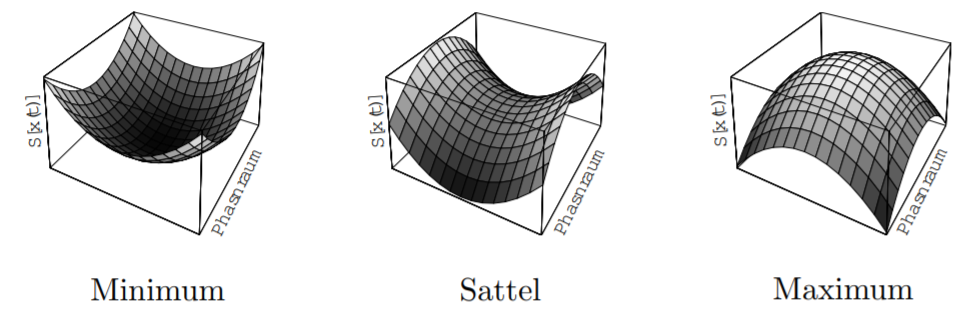
\includegraphics[scale=1]{1_10.PNG}
    \captionsetup{font={Large}}
    \caption{Different extremes of the effect $S[x(t)]$ in the phase space}
    \label{fig:1.10}
\end{figure}
\subsection{Quantum Mechanics}
According to Heisenberg's principle of blur, we can not fix $x (t)$. The blur is in effect and of the order of magnitude $h$, the effect quantum. From this one can assume that the relevant parameters is the dimensionless effect $S / h$. Next we search
a complex amplitude $\Phi[x (t)] \in C$ for the path $x (t)$. This amplitude describes the wave character of the particle, which is why we use a dimensionless
Need phase $\phi[x (t)]$. The approach $\phi[x (t)]/2\pi = S/h$ for the phase gives the amplitude
\\
\begin{equation}
\Phi[x(t)] \sim e^{i \mathcal{S}[x(t)] / \hbar}
\end{equation}\\
%公式1.11
for the path $x (t)$. Note that this is not a derivation of quantum mechanics
is. The following correspondences result(In addition, from later versions or the textbooks of Messiah,
p. 222, as well as Fetter, Walecka, p. 184, see also the Hamilton-Jakobi formalism in the
Mechanics or the quasi-classical approximation in Chap. 10)
\\
\begin{equation}
\begin{array}{c}{\text { quantum mechanics } \cong \text { wave optics }} \\ 
{\qquad \begin{aligned} 
\hbar\to 0 \downarrow \text { Approximation } & \text { Eikonalapprox } \downarrow \lambda \rightarrow 0 \\ \text { classical mechanics } & \cong \text { geometric appearance } \end{aligned}}\end{array}
\end{equation}\\
%公式1.12
%PAGE 25
\\
The combination of (1.8) and (1.11) gives the amplitude $K (b, a)$
which describes the propagation of a particle from $a$ to $b$
\\\begin{equation}
K(b, a)=\sum_{x(t)} \Phi[x(t)]
\end{equation}\\
%公式1.13
and for the (relative) probability $P (b, a)$ that the particle is undisturbed
from $a$ to $b$ (ie without destroying the interference)\\
\begin{equation}
P(b, a)=|K(b, a)|^{2}
\end{equation}\\
%公式1.14
$K (b, a)$ is called the \textbf{propagator} and describes the 'movement' of the particle of
$a$ to $b$.
%图1.11
\begin{figure}[ht]
    \centering
    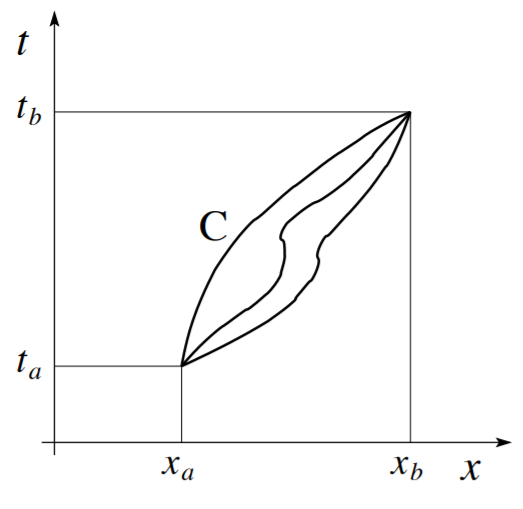
\includegraphics[scale=1]{1_11.PNG}
    \captionsetup{font={Large}}
    \caption{In the path integral is summed over all paths $C$ beginning in $a = (xa, ta)$ and ending in $b = (xb, tb)$.}
    \label{fig:1.11}
\end{figure}
\\\textbf{Classic Limes}\\\\
Consider (1.13). Now suppose that the typical effect $S [x (t)]$
for $x (t)$ from $a$ to $b$ of the order of magnitude S0 let. $S_0 / h$ then gives the
Phase rotation in amplitude to the path from $a$ to $b$. If $S_0$ big
is, generic adjacent paths $x (t)$ and $x (t) + \delta x (t)$
already many revolutions, that is, they are strongly out of phase and
therefore interfere destructively; their sum is small. Only special paths with
Deviations $\delta S_0/h \ll 1$ contribute to $K (b, a)$; such paths are close by
of the classical path where $\delta S [\bar{x} (t)] = 0$, that is, the relevant trajectory
the classical, $\bar{x} (t)$. For big $S_0$ (big masses, big energies, ...)
only the very nearest environment of the classical path $\bar{x} (t)$ to the integral and we discover the results of classical physics; also goes for $h\to 0$ quantum mechanics into classical mechanics.
%PAGE 26
Semi-classical approximation: in the semi-classical approximation
let's write the propagator as a product of a volume factor and
a phase factor, the latter via the effect over the classical
Path is evaluated,
\\
\begin{equation}
K(b, a)=V(b) e^{i \mathcal{S}[\bar{x}] / \hbar}
\end{equation}\\
%公式 1.15
The volume factor $V (b)$ is a smooth function; the strong variation with the
Change of the end point b is in the phase factor $e^{iS[\bar x]/\bar{h}}$. The name
'half-classic' refers to the description of the particle (system) via
a wave function whose phase is determined by the classical effect
is. $V (b)$ indicates the volume of the paths which contribute to $K$,
see. Figure 1.12.
%图 1.12
\begin{figure}[ht]
    \centering
    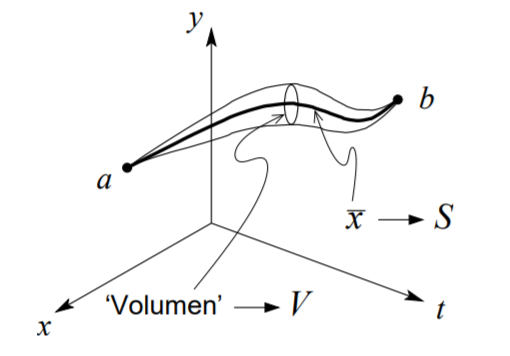
\includegraphics[scale=1]{1_12.PNG}
    \captionsetup{font={Large}}
    \caption{In the semi-classical approximation, the propagator $K (b, a)$ results as a product of a volume factor $V (b)$ and a phase factor $exp [iS [\bar{x}]/\hbar]$ with an effect $S$ evaluated over the classical path $\bar{x}(t)$.}
    \label{fig:1.12}
\end{figure}
\\
\textbf{Summation over paths}\\\\
The Riemann integral over a function $f (x)$ is defined as a limit the Riemann sum
\\
\begin{equation}
\lim _{\eta \rightarrow 0}\left[\eta \sum_{i} f\left(x_{i}\right)\right]
\end{equation}\\
%公式 1.16
where the measure is given by the 'breadth' of an interval, cf. Illustration
1.13. Similarly, we de nieren a sum of paths by
Discretize time and space, and take the appropriate limit, cf.
Figure 1.13. For each time step $t_i$, we sum over all possible positions $x_i$,
\\
\begin{equation}
K(b, a)=\lim _{\varepsilon \rightarrow 0} \frac{1}{A} \int_{-\infty}^{\infty} \frac{d x_{1}}{A} \int_{-\infty}^{\infty} \frac{d x_{2}}{A} \cdots \int_{-\infty}^{\infty} \frac{d x_{N-1}}{A} e^{i \mathcal{S}[x(t)] / \hbar}
\end{equation}\\
%公式 1.17
It raises the question of the value of Mass A. As this constant
is universal (analogous to the Riemann integral), it satisfies the path integral
%PAGE27
%Figure 1.13
\begin{figure}[ht]
    \centering
    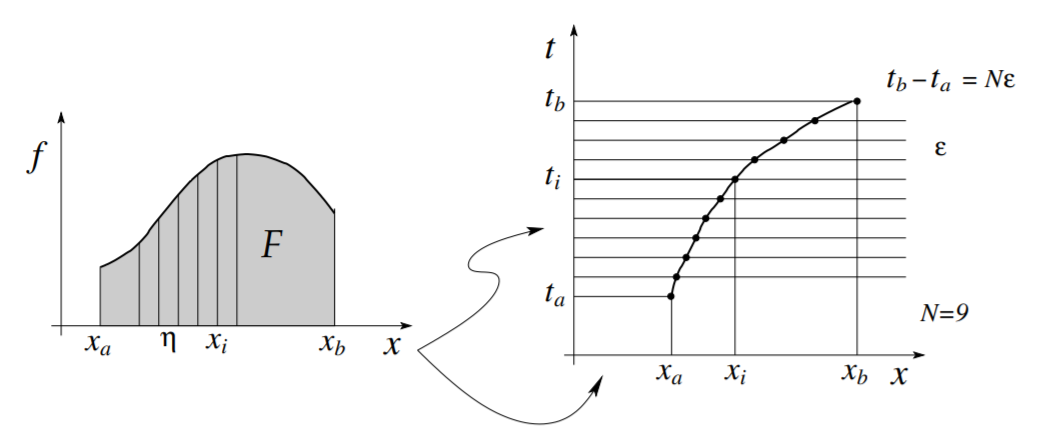
\includegraphics[scale=1]{1_13.PNG}
    \captionsetup{font={Large}}
    \caption{Left: Riemann integral with support points $x_i$ in the distance. Right: In the path integral is summed over all paths that connect $a = (xa, ta)$ to $b = (xb, tb)$. In this case, both the $x$-axis and the time $t$ are discretized, with intervals $dx$ (as in the Riemann integral) in place and $\epsilon$ in the time interval. $\epsilon$ defines the measure $A=\sqrt{2\pi i\hbar\epsilon/m}$}
    \label{fig:1.13}
\end{figure}
for a simple case. We consider a free particle,
\\
$$
\mathcal{L}(x, \dot{x}, t)=\mathcal{L}(\dot{x})=\frac{m}{2} \dot{x}^{2} \approx \frac{m}{2}\left(\frac{x_{i+1}-x_{i}}{\varepsilon}\right)^{2}
$$\\
%公式
and generally, $\mathcal{L}[(x_{i + 1} + x_i) = 2, (x_{i + 1}- x_i) /\epsilon, (t_{i + 1} + t_i) / 2]$. In the discretized
Form we can calculate the occurring integrals,
\\
$$
\begin{aligned} 
K(b, a)= & \lim _{\varepsilon \rightarrow 0} A^{-N}\left[\prod_{i=1}^{N-1} \int d x_{i}\right] e^{\frac{i m}{2 \hbar} \varepsilon \sum_{j=0}^{N-1}\left(\frac{x_{j+1}-x_{j}}{\varepsilon}\right)^{2}} 
\\
= & \lim _{\varepsilon \rightarrow 0} A^{-N}\left[\prod_{i=2}^{N-1} \int d x_{i}\right] 
\begin{array}
    {l}{\frac{i m}{2 \hbar \varepsilon} \sum_{j=2}^{N-1}\left(x_{j+1}-x_{j}\right)^{2}}
\end{array} 
\\ 
%\qquad \begin{aligned}
= & 2\left[x_{1}-\left(x_{2}+x_{a}\right) / 2\right]^{2}+x_{2}^{2}+x_{a}^{2}-\left(x_{2}+x_{a}\right)^{2} / 2 
\\
= & 2\left[x_{1}-\left(x_{2}+x_{a}\right) / 2\right]^{2}+\left(x_{2}-x_{a}\right)^{2} / 2 
\\ \rightarrow & \sqrt{\frac{\pi i \hbar 2 \varepsilon}{2 m}} e^{\frac{i m}{2 h(2 \varepsilon)}\left(x_{2}-x_{a}\right)^{2}} %\end{aligned} 
\end{aligned}
$$\\
$$
\downarrow \text { mit Gauss: } \int d x e^{i a x^{2}}=\sqrt{\frac{i \pi}{a}} \text { und } \int d x e^{-\frac{x^{2}}{2 \sigma}}=\sqrt{2 \pi \sigma}
$$
$$\\
\begin{aligned}=\lim _{\varepsilon \rightarrow 0} A^{-N}\left(\frac{2 \pi i \hbar \varepsilon}{2 m}\right)^{1 / 2} &\left[\prod_{i=3}^{N-1} \int d x_{i}\right] e^{\frac{i m}{2 \hbar \varepsilon} \sum_{j=3}^{N-1}\left(x_{j+1}-x_{j}\right)^{2}} \\ & \times \underbrace{\int d x_{2} e^{\frac{i m}{2 \hbar \varepsilon}\left[\left(x_{3}-x_{2}\right)^{2}+\frac{1}{2}\left(x_{2}-x_{a}\right)^{2}\right]}}_{\sqrt{\frac{2 \pi i \hbar 2 \varepsilon}{3 m}} e^{\frac{i m}{2 \hbar(3 \varepsilon)}}\left(x_{3}-x_{a}\right)^{2}} \end{aligned}
$$\\
$$
\begin{aligned} &=\lim _{\varepsilon \rightarrow 0} A^{-N}\left(\frac{2 \pi i \hbar \varepsilon}{m}\right)^{(N-1) / 2} \frac{1}{\sqrt{2}} \cdot \sqrt{\frac{2}{3}} \cdot \sqrt{\frac{3}{4}} \cdots \\ &=\lim _{\varepsilon \rightarrow 0} \frac{1}{A}\left(\frac{2 \pi i \hbar \varepsilon}{A^{2} m}\right)^{(N-1) / 2} \sqrt{\frac{\varepsilon}{\varepsilon N}} e^{\frac{i m}{2 \hbar\left(t_{b}-t_{a}\right)}\left(x_{b}-x_{a}\right)^{2}} \end{aligned}
$$\\
\begin{equation}
\begin{array}{l}{\downarrow \Rightarrow A=\sqrt{\frac{2 \pi i \hbar \varepsilon}{m}}} \\ {=\sqrt{\frac{m}{2 \pi i \hbar\left(t_{b}-t_{a}\right)}} \exp \left[\frac{i m\left(x_{b}-x_{a}\right)^{2}}{2 \hbar\left(t_{b}-t_{a}\right)}\right]}\end{array}
\end{equation}\\
%公式
With the simplified start and end coordinates $t_a = 0, t_b = t, x_a = 0$
and $x_b = x$ we ​​find the simpler form for K
\\
\begin{equation}
K(x, t)=\sqrt{\frac{m}{2 \pi i \hbar t}} \exp \left[\frac{i m x^{2}}{2 \hbar t}\right]
\end{equation}\\
%公式 1.19
Definition: under the path integral
\begin{equation}
K(b, a) \equiv \int_{a}^{b} \mathcal{D}[x(t)] e^{i S[x(t)] / \hbar}
\end{equation}
%公式 1.20
one understands the expression
\\
\begin{equation}
\begin{aligned} K(b, a) &=\lim _{\varepsilon \rightarrow 0}\left(\frac{m}{2 \pi i \hbar \varepsilon}\right)^{N / 2} \int_{-\infty}^{\infty} \prod_{i=1}^{N-1} d x_{i} \\ & \times \exp \left[\frac{i \varepsilon}{\hbar} \sum_{j=0}^{N-1} \mathcal{L}\left(\frac{x_{j+1}+x_{j}}{2}, \frac{x_{j+1}-x_{j}}{\varepsilon}, \frac{t_{j+1}+t_{j}}{2}\right)\right] \end{aligned}
\end{equation}\\
%公式 1.21
where $N = (t_b - t_a) /\epsilon, (x_0, t_0) = a$ and $(x_N, t_N) = b$.
%PAGE 29
An illustration of the propagator $K (x, t)$ of the free particle (1.19) is in the
Figures 1.14 and 1.15 given; These suggest the de nition of one
local wavelength $\lambda$ and a local period $T$. The local wavelength is $\lambda$
%Figure  1.14
\begin{figure}[ht]
    \centering
    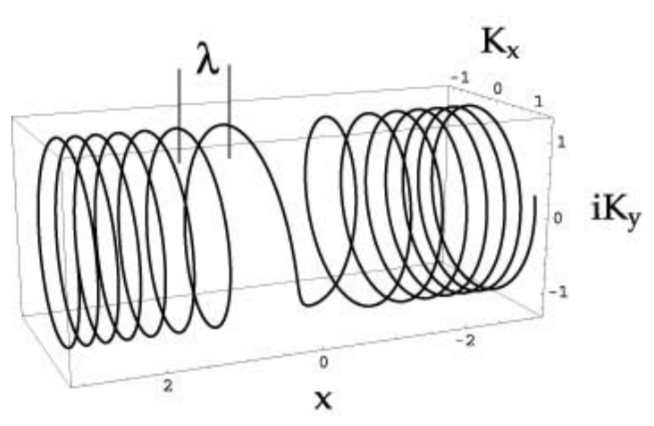
\includegraphics[scale=1]{1_14.PNG}
    \captionsetup{font={Large}}
    \caption{$K (x, t)$ for the free particle as a function of $x$ at fixed $t$ leads to the definition of a local wave with increasing
    distance $x$ decreases.}
    \label{fig:1.14}
\end{figure}
, see Figure 1.14 can be found in the approximation of large distances $x\gg \lambda$
calculate as
\\
\begin{equation}
\begin{aligned} m \frac{(x+\lambda)^{2}-x^{2}}{2 \hbar t} &=\frac{m x \lambda}{\hbar t}\left(1+\frac{\lambda}{2 x}\right)=2 \pi \\ \lambda & \stackrel{x \gg \lambda}{=} \frac{h}{m v}=h / p \end{aligned}
\end{equation}\\
%公式 1.22
$\Rightarrow$ Particles which contribute to $K$ in $x$ at time $t$ have the
Impuls $p = mx / t$ and are quantum mechanically as a wave with $\lambda = h/p$
described.
The local period T (Figure 1.15) may be longer in the approximation
Times $t\gg T$ determine
\\
\begin{equation}
\frac{m x^{2}}{2 \hbar}\left(\frac{1}{t}-\frac{1}{t+T}\right)=\frac{m x^{2}}{2 \hbar t^{2}}\left(\frac{T}{1+T / t}\right)=2 \pi
\end{equation}\\
%公式 1.23
Particles that contribute to $K$ in $x$ at time $t$ have the energy $E = m (x / t)^2 / 2$ and are quantum mechanically as wave with period $T = h / E$ described. The angular frequency of the wave is given by
\\
\begin{equation}
\omega=\frac{2 \pi}{T} \stackrel{t \gg T}{=} \frac{1}{\hbar} \frac{m}{2}\left(\frac{x}{t}\right)^{2}=\frac{E}{\hbar}
\end{equation}\\
%公式 1.24
%PAGE 30
%Figure  1.15
\begin{figure}[ht]
    \centering
    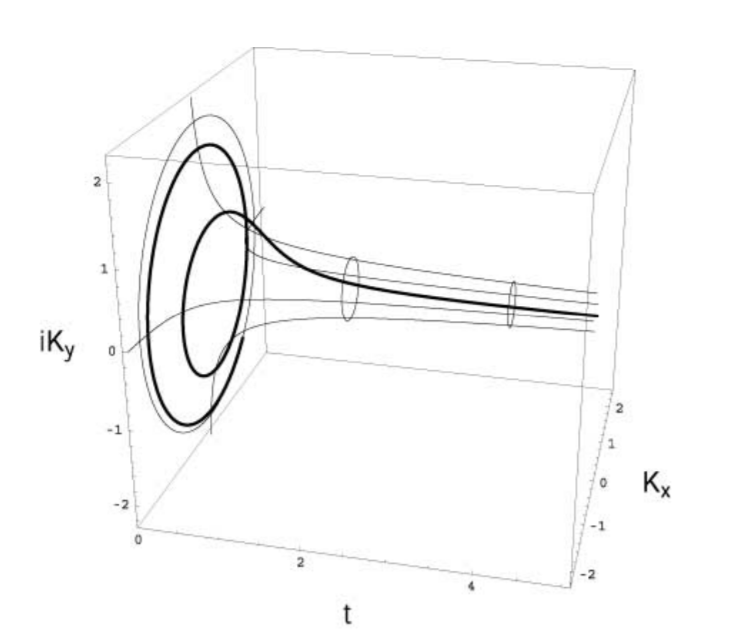
\includegraphics[scale=1]{1_15.PNG}
    \captionsetup{font={Large}}
    \caption{$K (x, t)$ for the free particle as a function of $t$ at fixed $x$, allows the definition of a local period $T$ which increases with increasing time.}
    \label{fig:1.15}
\end{figure}
\\
In general, we can have any propagator K in the semi-classical
Approximation $K (b, a) \sim exp [iS_{kl}(b, a)/\hbar]$ by a local wave and
describe a local period: the dominant dependency of $K (b)$
appears in the phase factor and allows the definition of the local wave
and the local period according to
\\
\begin{equation}
\begin{array}{l}{h=2 \pi \hbar=S_{k l}\left(x_{b}+\lambda\right)-S_{k l}\left(x_{b}\right)=\lambda \frac{\partial S_{k l}}{\partial x_{b}}=\lambda p} \\ {h=2 \pi \hbar=S_{k l}\left(t_{b}+T\right)-S_{k l}\left(t_{b}\right)=T \frac{\partial S_{k l}}{\partial t_{b}}=T E}\end{array}
\end{equation}\\
%公式 1.25
\subsection{Product rule}
The propagator $K (b, a)$ is derived from partial propagations over subintervals
$(a, c)$ and $(c, b)$ are composed, whereby over all positions of the
Intermediate point $c$ is to sum, cf. Figure  1.16. The Additivit of the
Effect in the exponent leads to the product of the partial propagators; the
Factorization in subpaths can be repeated iteratively,
\\
\begin{equation}
\begin{split}
K(b,a)&
=\int \mathcal{D}[x(t)] e^{(i / \hbar)[S(b, c)+S(c, a)]} \\
&=\int d x_{c} K(b, c) K(c, a) \\ 
&=\int \prod_{i=1}^{N-1} d x_{i} K\left(b, x_{N-1}\right) K\left(x_{N-1}, x_{N-2}\right) \cdots K\left(x_{1}, x_{a}\right)
\end{split}
\end{equation}\\
%公式 1.26

%PAGE 31
%Figure  1.16
\begin{figure}[ht]
    \centering
    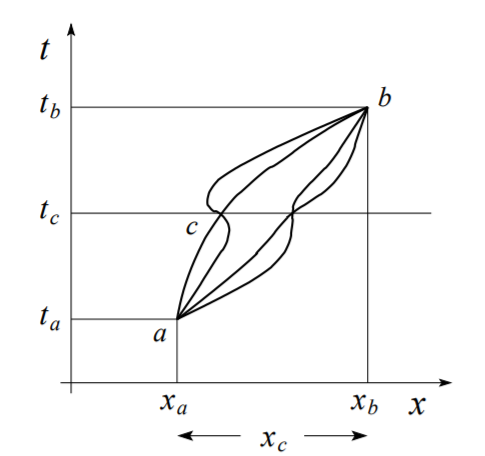
\includegraphics[scale=1]{1_16.PNG}
    \captionsetup{font={Large}}
    \caption{Illustration of the product rule with an intermediate step at $t_c$.}
    \label{fig:1.16}
\end{figure}
\subsection{Wave function}
$K (b, a)$ describes the propagation of a particle from $a$ to $b$. We generalize
this result by looking at a particle of which
we do not have its initial position (at a) but only the amplitude $\Psi(a) = \Psi(x_a, t_a)$ know. Then according to (1.26) the following amplitude results in $b$,
\begin{equation}
\Psi\left(x_{b}, t_{b}\right)=\int_{-\infty}^{\infty} d x_{a} K\left(x_{b}, t_{b} ; x_{a}, t_{a}\right) \Psi\left(x_{a}, t_{a}\right)
\end{equation}
%公式 1.27
the wave function of the particle at a later time $t_b$. $|\Psi (x_b, t_b)|^2$
is the (relative) probability of finding the particle in $x_b$ at time $t_b$.
Note: The knowledge of $\Psi$ at one time (here $t_a$) determines $\Psi$ for all times.
This results in a differential equation of the first order for the time evolution
in $d / dt$.
In classical mechanics two initial conditions $x$ and $\partial_t x$ are required,
to set the particle trajectory. That is why in the classic
Mechanics a di erential equation 2nd order in $d / dt$ from ot.

%PAGE 32
\section{Generalizations}
We consider three generalizations for the propagator $K$, the particle
in the potential $V (x)$, the particle in the multidimensional space $\mathbb{R}^n$, and
the propagator for several particles.

\subsection{Particles in the potential $V (x)$}
We can exactly determine the propagator $K$ if and only if the Lagrange function
$\mathcal{L} (x, \dot{x}, t)$ is a 2nd order polynomial in $x$ and $\dot{x}$. The reason
This restriction is that we only calculate Gauss integrals
k may. It was
\\
\begin{equation}
\mathcal{L}=a \dot{x}^{2}+b \dot{x} x+c x^{2}+d \dot{x}+e x+f
\end{equation}\\
%公式 1.28
wanted is $K$,
\\
\begin{equation}
K(b, a)=\int_{a}^{b} \mathcal{D}[x(t)] \exp \left[\frac{i}{\hbar} \int_{t_{a}}^{t_{b}} d t \mathcal{L}(x, \dot{x}, t)\right]
\end{equation}\\
%公式 1.29
Moody way: as before on page 28. Easier: Let $\delta S(\bar{x}) = 0$, with the
classical path $\bar{x}$. Then with $x = \bar{x} + y$,
\\
\begin{equation}
S[x(t)]=S[\bar{x}(t)]+\int_{t_{a}}^{t_{b}} d t\left[a \dot{y}^{2}+b \dot{y} y+c y^{2}\right]
\end{equation}\\
%公式 01.30
the contributions of the terms linear in $y$ and $\dot{y}$ vanish because $\delta S (\bar{x}) = 0$. Thus
we will
\\
\begin{equation}
\begin{aligned} K(b, a) &=\exp \left[\frac{i}{\hbar} S[\bar{x}(t)]\right] \int_{0}^{0} \mathcal{D}[y(t)] \exp \left[\frac{i}{\hbar} \int_{t_{a}}^{t_{b}} d t\left[a \dot{y}^{2}+b \dot{y} y+c y^{2}\right]\right] \\ &=\exp \left[\frac{i}{\hbar} S[\bar{x}(t)]\right] F\left(t_{b}, t_{a}\right) \end{aligned}
\end{equation}\\
%公式 1.31
a development around the classical way. The whole dependency of
the positions $x_a, x_b$ appears in the exponential factor via the classic
Path $\bar{x}(t)$.
Now let $\mathcal{L} = T - V$, as known from classical mechanics. Then
we write again
\\
\begin{equation}
\begin{aligned} V(x) &=V(\bar{x}+y)=V(\bar{x})+y V^{\prime}(\bar{x})+\frac{y^{2}}{2} V^{\prime \prime}(\bar{x})+\frac{y^{3}}{6} V^{\prime \prime \prime}(\bar{x})+\cdots \\ & \downarrow \text { quadratische Approximation } \\ & \cong V(\bar{x})+y V^{\prime}(\bar{x})+\frac{y^{2}}{2} V^{\prime \prime}(\bar{x}) \end{aligned}
\end{equation}\\
%公式 1:32
%PAGE 33
That's how we get
\\
\begin{equation}
\begin{aligned} K(b, a) & \cong \exp [i S[\bar{x}(t)] / \hbar] \\ & \times \int_{0}^{0} \mathcal{D}[y(t)] \exp \left[\frac{i}{\hbar} \int_{t_{a}}^{t_{b}} d t\left(\frac{m}{2} \dot{y}^{2}-\frac{m \omega^{2}}{2} y^{2}\right)\right] \end{aligned}
\end{equation}\\
%公式 1:33
with $w^2 = V^{''}(\bar{x}(t))/m$ analogous to the harmonic oscillator. This approximation
is good if one of the following points is true:
\{$S/\hbar \gg 1$, then y is small and $y^3$ is negligible.
\{$V$ square, so (1.33) is exact.
\{$V$ smooth, so $V^{(n)}$ for $n\geq 3$ is small$\to$ WKB (Wenzel-Kramers Brillouin).
\{$tb - ta$ small and thus $y$ is small because otherwise $T$ is big.
1.3.2 Particles in marg
The definition (1.20) of the path integral for $n = 1$ is immediately apparent
Generalize movements in high dimensional spaces,
\\
\begin{equation}
\begin{aligned} K(\vec{b}, \vec{a})=& \int_{\vec{a}}^{\vec{b}} \mathcal{D}[\vec{r}(t)] \exp (i S[\vec{r}(t)] / \hbar) \\ & \quad \operatorname{mit} \mathcal{D}[\vec{r}(t)]=\mathcal{D}\left[x_{1}(t)\right] \cdots \mathcal{D}\left[x_{n}(t)\right] \end{aligned}
\end{equation}\\
%公式 1:34
that is, the path integral involves a factor for each dimension. Note
that the problem is generally not factored; the movements in the
different directions are not independent.
1.3.3 Several particles
Again, the generalization is immediately obvious: again occurs
a product of path integrals, similar to 1.3.2. For $k$ particles that
propagate from $\vec{ak}$ to $\vec{bk}$, let the propagator write as
\\
\begin{equation}
\begin{aligned} K\left(\vec{b}_{1}, \cdots, \vec{b}_{k} ; \vec{a}_{1}, \ldots, \vec{a}_{k}\right)=& \int_{\vec{a}_{1}}^{\vec{b}_{1}} \mathcal{D}\left[\vec{r}_{1}(t)\right] \cdots \int_{\vec{a}_{k}}^{\vec{b}_{k}} \mathcal{D}\left[\vec{r}_{k}(t)\right] \\ & \times \exp \left[\frac{i}{\hbar} S\left[\vec{r}_{1}(t), \ldots, \vec{r}_{k}(t)\right]\right] \end{aligned}
\end{equation}\\
%公式 1:35
%PAGE 34
For two interacting particles in the $\mathbb{R}^1\times \mathbb{R}^1$ with the Lagrangian
\\
\begin{equation}
\mathcal{L}=\frac{m}{2} \dot{x}^{2}+\frac{M}{2} \dot{X}^{2}-V(x, X, t)
\end{equation}\\
%公式 1:36
If you find the propagator,
\\
\begin{equation}
\begin{array}{c}{K\left(x_{b}, X_{b}, t_{b} ; x_{a}, X_{a}, t_{a}\right)=\int \mathcal{D}[x(t)] \mathcal{D}[X(t)] \exp \left[\frac{i}{\hbar} S[x(t), X(t)]\right]} \\ {=\int \mathcal{D}[x(t)] \exp \left[\frac{i}{\hbar} \int_{t_{a}}^{t_{b}} \frac{m}{2} \dot{x}^{2} d t\right] T[x(t)]}\end{array}
\end{equation}\\
%公式 1:37
with the functional $T [x (t)]$ given as a path integral over the coordinate
$X (t)$ of the other particle (the In
uenzintegral)
\\
\begin{equation}
T[x(t)]=\int \mathcal{D}[X(t)] \exp \left[\frac{i}{\hbar} \int_{t_{a}}^{t_{b}}\left[M \dot{X}^{2} / 2-V(x, X, t)\right]\right]
\end{equation}\\
%公式 1:38
If $V = V_x (x) + V_X(X)$, so no interaction takes place, then
separates the system and
\\
\begin{equation}
K\left(x_{b}, X_{b}, t_{b} ; x_{a}, X_{a}, t_{a}\right)=K_{x}\left(x_{b}, t_{b} ; x_{a}, t_{a}\right) \times K_{X}\left(X_{b}, t_{b} ; X_{a}, t_{a}\right)
\end{equation}\\
%公式 1:39
Dissipative Problems: In classical mechanics, a particle can be found
describe with friction by the dissipative dynamics $m\ddot{x}+\eta\dot{x}=-\partial_xV(x)$
the term $\eta\dot{x}$ describes the friction and implies that energy
is dissipated. The quantum mechanical description of this problem is
difficult because we have to resort to a Hamiltonian formulation.
Feynman and Vernon and later Caldeira and Leggett have suggested
to couple the system to a reservoir of harmonic oscillators
and then to integrate over the coordinates of the oscillators, cf.
Figure  1.17. The total system particles \& reservoir is by the Lagarian
%Figure  1.17
\begin{figure}[ht]
    \centering
    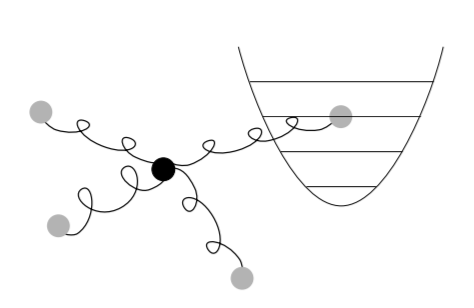
\includegraphics[scale=1]{1_17.PNG}
    \captionsetup{font={Large}}
    \caption{Description of a dissipative system: the coordinate is coupled to a reservoir of harmonic oscillators, which is then integrated.}
    \label{fig:1.17}
\end{figure}

%PAGE 35
%\\
\begin{equation}
\begin{array}{r}{\mathcal{L}=\frac{m}{2} \dot{x}^{2}-V(x)+\sum_{k}\left(\frac{M_{k}}{2} \dot{X}_{k}^{2}-\frac{M_{k} \omega_{k}^{2}}{2} X_{k}^{2}\right)} \\ {-\underbrace{\sum_{k} q_{k} x X_{k}}_{\text {lin. Koplung }}-\underbrace{\sum_{k} \frac{q_{k}^{2} x^{2}}{2 M_{k} \omega_{k}}}_{\text {Gegenterm }}}\end{array}
\end{equation}\\
%公式 1:40
described. The interaction is via the linear coupling term
$xX_k$ takes place; the counter-guarantor guarantees that the potential $V (x)$ through the bath
is not renormalized. After integration over the reservoir degrees of freedom
$X_k$ is the e ff effective propagator
\\
\begin{equation}
\begin{aligned} K\left(x_{b}, t_{b} ; x_{a}, t_{a}\right) &=\int \mathcal{D}[x(t)] \exp \left[\frac{i}{\hbar} S_{\mathrm{eff}}[x(t)]\right] \\ S_{\mathrm{eff}} &=\int d t\left[\frac{m}{2} \dot{x}^{2}-V(x)+\text { Dissipativer Term }\right] \end{aligned}
\end{equation}\\
%公式 1:41
Further details can be found in R.P. Feynman and F.L. Vernon, Annals of
Physics 24, 118 (1963) and in A.O. Caldeira and A.J. Leggett, Annals of
Physics 149, 374 (1983). (The work of Feynman and Vernon deals with the problem of real-time dynamics,
while Caldeira and Leggett are experiencing quantum statistical problems in the imaginary artefact
Discuss formalism.)

\section{Schrodinger equation}
We start from the relation (1.27), which is the evolution of the wave function
of a particle describes
\\
\begin{equation}
\Psi\left(x_{b}, t_{b}\right)=\int_{-\infty}^{\infty} d x_{a} K\left(x_{b}, t_{b} ; x_{a}, t_{a}\right) \Psi\left(x_{a}, t_{a}\right)
\end{equation}\\
%公式 1:42
it describes the dynamics of the system in an integral way. We
seek a di erential form of dynamics. Since (1.42) holds for all $t_b> t_a$,
we can choose $t = t_a$ and $t_b = t + \epsilon$ and with $\mathcal{L}=(m/2)\dot{x}^2-V(x,t)$
we receive
\\
\begin{equation}
\begin{aligned} \Psi(x, t+\varepsilon) &=\int \frac{d y}{A} \exp \left[\frac{i}{\hbar} \varepsilon \mathcal{L}\left(\frac{x+y}{2}, \frac{x-y}{\varepsilon}, t+\frac{\varepsilon}{2}\right)\right] \Psi(y, t) \\ &=\int \frac{d y}{A} \exp \left[\frac{i m}{2 \hbar \varepsilon}(x-y)^{2}\right] \exp \left[-\frac{i \varepsilon}{\hbar} V\left(\frac{x+y}{2}, t+\frac{\varepsilon}{2}\right)\right] \Psi(y, t) \end{aligned}
\end{equation}\\
%公式 1:43
%PAGE 36
It must be $x-y$ small, otherwise $T = m\dot{x}^2/2$ large. We de fi ne $y = x +\eta$,
with small, and $\eta$
\\
\begin{equation}
\Psi(x, t+\varepsilon)=\int \frac{d \eta}{A} \exp \left[\frac{i m \eta^{2}}{2 \hbar \varepsilon}\right] \exp \left[-\frac{i \varepsilon}{\hbar} V(x+\eta / 2, t+\varepsilon / 2)\right] \Psi(x+\eta, t)
\end{equation}\\
%公式 1:44
For $m\eta^2/2\hbar\epsilon>1$ the first factor oscillates strongly and thus cuts the
$\eta$-Integration ectively at
$\eta \sim \sqrt{\epsilon \hbar/m}$, we get a consistent one $\epsilon$ Development alright "if we develop to potencies $\epsilon$ and $\eta^2$,
\\\begin{equation}
\begin{aligned} \Psi(x, t)+\varepsilon \partial_{t} \Psi(x, t) \cong \int_{-\infty}^{\infty} \frac{d \eta}{A} \exp \left(\frac{i m \eta^{2}}{2 \hbar \varepsilon}\right)\left[1-\frac{i \varepsilon}{\hbar} V(x, t)\right] \\ \times\left[\Psi(x, t)+\eta \partial_{x} \Psi(x, t)+\frac{\eta^{2}}{2} \partial_{x}^{2} \Psi(x, t)\right] \end{aligned}
\end{equation}
\\
%公式 1:45
The evolution into orders of $\epsilon$ yields
$\epsilon^0$ terms:
\\
\begin{equation}
\begin{aligned} \Psi(x, t) &=\int_{-\infty}^{\infty} \frac{d \eta}{A} \exp \left(\frac{i m \eta^{2}}{2 \hbar \varepsilon}\right) \Psi(x, t) \\ &=\sqrt{\frac{2 \pi i \hbar \varepsilon}{m}} \frac{1}{A} \Psi(x, t) \\ \Rightarrow A &=\sqrt{\frac{2 \pi i \hbar \varepsilon}{m}} \end{aligned}
\end{equation}\\
%公式 1:46
This is the easiest way to find A.\\
$\epsilon^{1/2}$ terms:
\\
\begin{equation}
0=0 \quad\left(\int_{-\infty}^{\infty} d \eta \eta \exp \left[\frac{i m \eta^{2}}{2 \hbar \varepsilon}\right]=0\right)
\end{equation}\\
$\epsilon^1$ terms:
\\
\begin{equation}
\varepsilon \partial_{t} \Psi(x, t)=\underbrace{\int_{-\infty}^{\infty} \frac{d \eta}{2 A} \eta^{2} \exp \left[\frac{i m \eta^{2}}{2 \hbar \varepsilon}\right]}_{i \hbar \varepsilon / 2 m} \partial_{x}^{2} \Psi+\frac{\varepsilon}{i \hbar} V(x, t) \Psi(x, t)
\end{equation}\\
%公式 1:48
This gives us the Schrodinger equation
\\
\begin{equation}
i \hbar \partial_{t} \Psi=-\frac{\hbar^{2}}{2 m} \partial_{x}^{2} \Psi+V(x, t) \Psi
\end{equation}\\
%公式 1:49
%PAGE 37
\\\textbf{Remarks}\\
1. The Schrodinger equation (1.49) is a 1-th order differential equation, thus satisfies $\Psi(xm t = t_0)$ as an initial condition.\\
2. The time derivative $i\hbar \partial_t$ defines a Hamiltonian dynamics, which of the dissipative dynamics $\partial_t \Psi=D\partial^2_x\Psi$ is the Diffusion different (A typical example of the equation of the equation is that for the temperature T, that is, $\Psi(x, t) = T (x, t)$.\\
3. $K (x_2, t_2; x_1, t_1) = K (2; 1)$ is a solution of the Schr odinger equation
(1.49) for $t_2> t_1$:
\\
\begin{equation}
i \hbar \partial_{t_{2}} K(2,1)=-\frac{\hbar^{2}}{2 m} \partial_{x_{2}}^{2} K(2,1)+V(2) K(2,1)
\end{equation}\\
%公式 1:50
Further, $K (2, 1) = K (x_2, t_2; x_1, t_1)\to \delta(x_2 - x_1)$ for $t_2\to t_1^+$ (use
(1.42)). We define $K (2, 1)\equiv 0$  for $t_2 <t_1$. Then $K$ is the
Green's function to 1.49,
\\
\begin{equation}
\underbrace{\left[i \hbar \partial_{t_{2}}+\frac{\hbar^{2}}{2 m} \partial_{x_{2}}^{2}-V\left(x_{2}, t_{2}\right)\right]}_{\text {Schrödinger }} \underbrace{K(2,1)}_{\text {Green }}=i \hbar \delta\left(x_{2}-x_{1}\right) \delta\left(t_{2}-t_{1}\right)
\end{equation}\\
%公式 1:51
4. (1.49) describes particle waves in free space (potential $V = 0$).
these are plane waves, for example, in one dimension.
\\
\begin{equation}
e^{i(k x-\omega t)}
\end{equation}\\
%公式 1:52
This wave is in fact a solution of (1.49), being a dispersion the relationship $\hbar w=\hbar^2k^2/2m$. With (1.25) we get the correct dispersion $E=p^2/2m$ for a classical, massive, nonrelativistic one particles. For an alternative derivation of (1.49) you can start at $E=p^2/2m$ and the correspondence principle use $E\sim i\hbar\partial_t$ and $p\sim -i\hbar\partial_x$.\\
5. Dimension of (1.49): $[\hbar\partial_t]$ = Energy.\\
6. generalization to several dimensions, $x\to \vec{r}$,
\\
\begin{equation}
\begin{aligned} i \hbar \partial_{t} \Psi=& H \Psi \\ H &=-\frac{\hbar^{2}}{2 m} \nabla^{2}+V(\vec{r}, t) \\ \Psi &=\Psi(\vec{r}, t) \end{aligned}
\end{equation}\\
%公式 1:53
%PAGE 38
The expression $H$ is an operator, the Hamiltonian. The derivative $\triangledown$ acts on $\Psi$, the potential multiplied $\Psi$.
The Hamilton operator $H$ speaks about the principle of correspondence
(see later), using $\vec{p}\leftrightarrow -i\hbar\triangledown$. Other
Examples of operators are
\\
\begin{equation}
\begin{array}{l}{\vec{r}=\text { position operator }=\text { Multiplication with } \vec{r},} \\ {\vec{p}=\text { pulse operator }=\text { Derive after } \vec{r} .}\end{array}
\end{equation}\\
%公式 1:54
\section{Superposition principle}
The Schrodinger equation (1.49) is a linear differential equation.
If the solutions of the Schrodinger equation are $\Psi_i$, then these are also the functions
\\
\begin{equation}
\Psi=\sum_{i} a_{i} \Psi_{i}, \quad a_{i} \in \mathbb{C}
\end{equation}\\
%公式 1:55
The coefficients $a_i$ follow from the initial condition $\Psi(\vec{r}, t_0)$. We come back later. In the following we consider two simple one-dimensional
examples, the free particles and the particle in the \section{Free and bound particle}
\subsection{Free particles}
The Hamiltonian and the Schrödinger equation are given by
\\
\begin{equation}
H=-\frac{\hbar^{2}}{2 m} \partial_{x}^{2}, \quad i \hbar \partial_{t} \Psi(x, t)=-\frac{\hbar^{2}}{2 m} \partial_{x}^{2} \Psi(x, t)
\end{equation}
\\
%公式 1:56
We seek the general solution to any initial condition
$\Psi(x,0)$, analogous to (1.27). We can solve the problem by the separation approach
$\Psi_k(x,t)=\chi_k(t)\phi_k(x)$ solve,
\\
\begin{equation}
\begin{aligned} 
i \hbar \partial_{t} \chi_{k}=E_{k} \chi_{k}, & E_{k} \varphi_{k}=-\frac{\hbar^{2}}{2 m} \partial_{x}^{2} \varphi_{k} \\ \chi_{k}=\exp \left[-i \omega_{k} t\right], & \varphi_{k}=\exp (i k x), \quad k \in \mathbb{R} \\ E_{k} &=\hbar \omega_{k}=\hbar^{2} k^{2} / 2 m \end{aligned}
\end{equation}\\
%公式 1:57
%PAGE 39
The solutions $\phi_k(x)=e^{ikx}$ represent a basis. Note that particles
described by $\Psi_p(x,t)=e^{i(px-E_p(t)}$ the momentum p = \~{} k and the energy
$E_p=p^2/2m$, but since $|\Psi|^2=1$ are completely undetermined in place.
The initial value problem is solved by the superposition (1.58),
\\
\begin{equation}
\Psi(x, t)=\int \frac{d k}{2 \pi} a(k) \Psi_{k}(x, t)=\int \frac{d k}{2 \pi} a(k) e^{i\left(k x-\omega_{k} t\right)}
\end{equation}\\
%公式 1:58
From the initial condition at time $t = 0$ we can directly form (1.58)
Determine the amplitude $a (k)$,
\\
\begin{equation}
\begin{aligned} \Psi(x, 0)=\int \frac{d k}{2 \pi} a(k) e^{i k x} \Rightarrow a(k) &=\int d y \Psi(y, 0) e^{-i k y} \\ &=\int d y \Psi(y, 0) \Psi_{k}^{*}(y, 0) \end{aligned}
\end{equation}\\
%公式 1:59
and the time-dependent wave function $\Psi(x, t)$ results directly from the initial condition
via
\\
\begin{equation}
\Psi(x, t)=\int d y \int \frac{d k}{2 \pi} \Psi_{k}^{*}(y, 0) \Psi_{k}(x, t) \Psi(y, 0)
\end{equation}\\
%公式 1.60
For the propagator we find the expression
\\
\begin{equation}
\begin{aligned} K(x, t ; y, 0) &=\int \frac{d k}{2 \pi} \Psi_{k}^{*}(y, 0) \Psi_{k}(x, t) \\ &=\int \frac{d k}{2 \pi} e^{-i k y} e^{i\left(k x-\hbar k^{2} t / 2 m\right)} \\ &=\int \frac{d k}{2 \pi} \exp \left[-\frac{i \hbar t}{2 m}\left(k-\frac{(x-y) m}{\hbar t}\right)^{2}+\frac{i m(x-y)^{2}}{2 \hbar t}\right] \\ &=\sqrt{\frac{m}{2 \pi i \hbar t}} \exp \left[\frac{i m(x-y)^{2}}{2 \hbar t}\right] \end{aligned}
\end{equation}\\
%公式 1.61
Conforms to (1.19). Also note the completeness
$\int(dk/2\pi)\Psi^*_k(y,0)\Psi_k(x,0)=K(x-y, 0^+)=\delta(x-y))$ and orthogonality $\int dx\Psi^*_k(x,0)\Psi_{k'}(x,0)=2\pi \delta(k-k')$
\subsection{Particles in the 1D deep potential well}
The $\infty$ deep potential well is a potential free region of $\infty$ high surrounded walls, cf. Figure  1.18. For symmetry reasons one chooses the
%PAGE 40
%Figure  1.18
\begin{figure}[ht]
    \centering
    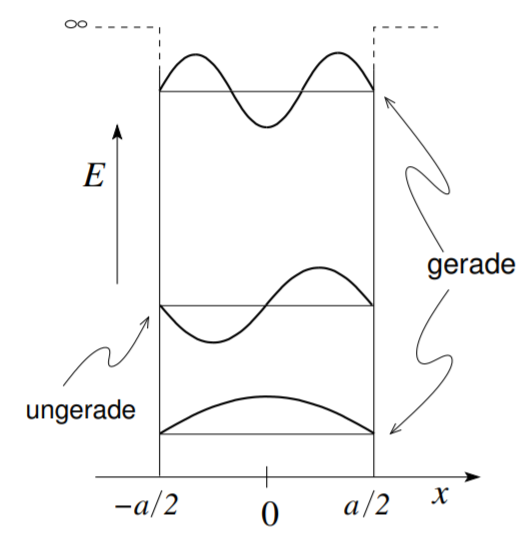
\includegraphics[scale=1]{1_18.PNG}
    \captionsetup{font={Large}}
    \caption{Conditions in the potential well with well-defined parity symmetry.}
    \label{fig:1.18}
\end{figure}
zero point in the middle. The system is characterized by the following Hamiltonian
description,
\\
\begin{equation}
\begin{aligned} H=-\frac{\hbar^{2}}{2 m} \partial_{x}^{2}+V_{\infty}(x) & \\ V_{\infty}(x) &=\left\{\begin{array}{ll}{0,} & {|x| \leq a / 2} \\ {\infty,} & {|x| \geq a / 2}\end{array}\right.\end{aligned}
\end{equation}\\
%公式 1.62
Again, one separates the problems in time and in place with the approach
\\
\begin{equation}
\Psi_{n}(x, t)=\chi_{n}(t) \varphi_{n}(x)
\end{equation}\\
%公式 1.63
we get the dynamic problem
\\
\begin{equation}
i \hbar \partial_{t} \chi_{n}=E_{n} \chi_{n}
\end{equation}\\
%公式 1.64
with the solution
\\
\begin{equation}
\chi_{n}=e^{-i \omega_{n} t}
\end{equation}\\
%公式 1.65
as well as the eigenvalue problem
\\
\begin{equation}
E_{n} \varphi_{n}=-\frac{\hbar^{2}}{2 m} \partial_{x}^{2} \varphi_{n}, \quad|x| \leq \frac{a}{2}
\end{equation}\\
%公式 1.66
with the boundary conditions
\\
\begin{equation}
\varphi_{n}(x) \equiv 0 \quad|x| \geq \frac{a}{2}
\end{equation}\\
%公式 1.67
%PAGE 41
The solutions are given by exponential functions $exp (\pm ikx)$, where
the allowed values ​​of $k$ are fixed by the boundary conditions,
\\\begin{equation}
k_{n}=n \frac{\pi}{a}
\end{equation}
\\
%gs 1.68
One finds solutions to even and odd $n$; these are odd resp.
straight in $x$,
\\
\begin{equation}
\varphi_{n}(x)=\left\{\begin{array}{ll}{\sin n \pi x / a,} & {n \geq 2, \quad \text { even }} \\ {\cos n \pi x / a,} & {n \geq 1, \quad \text { odd }}\end{array}\right.
\end{equation}\\
%公式 1.69
with the energies $E_n=\hbar^2 k_n^2/2m$(k-values ​​from the boundary conditions)
\\
\begin{equation}
E_{n}=\hbar \omega_{n}=\frac{\hbar^{2} k_{n}^{2}}{2 m}=\frac{\hbar^{2} \pi^{2}}{2 m a^{2}} n^{2}
\end{equation}\\
%公式 1.70
Again, the solution to the initial value problem is the superposition
\\
\begin{equation}
\Psi(x, t)=\sum_{n} a_{n} \Psi_{n}(x, t)
\end{equation}\\
%公式 1.71
given. For the initial condition to be fulfilled, must
\\
\begin{equation}
\begin{aligned} \Psi(x, 0)=& \sum_{n} a_{n} \Psi_{n}(x, 0) \\ & \stackrel{(1.59)}{\longrightarrow} a_{n}=\int d y \Psi(y, 0) \Psi_{n}^{*}(y, 0) \end{aligned}
\end{equation}\\
%公式 1.72
and thus one finds the following solution to the initial value problem,
\\
\begin{equation}
\Psi(x, t)=\int d y \sum_{n} \Psi_{n}^{*}(y, 0) \Psi_{n}(x, t) \Psi(y, 0)
\end{equation}\\
%公式 1.73
The propagator for the particle in the pot is
\\
\begin{equation}
\begin{aligned} K(x, t ; y, 0) &=\sum_{n} \Psi_{n}^{*}(y, 0) \Psi_{n}(x, t) \\ &=\sum_{n} \varphi_{n}^{*}(y) \varphi_{n}(x) e^{-i \omega_{n} t} \end{aligned}
\end{equation}\\
%公式 1.74
Of course, this solution strategy can also be applied to other problems
generalize, see later.
In the description of a free particle we note that plane
Waves basis $\Psi_k(x,t)$ is not normalizable. To mathematical problems
To avoid this, we must treat the wave functions more carefully; a
Possibility exists in the transition to wave packets, for example the
Gaussian wave packages.

%PAGE 42
\section{Gaussian Wave Packages}
Gaussian wave packages in place, i.e. Figure  1.19, describe particles in a localized state with finite extent $\triangle x$. Given that
Heisenberg Uncertainty Principle is the product $\triangle x\triangle k \sim 1$ fixed; a precise
localization in place then implies a broad distribution in the impulse (and
vice versa). Off the limes $\triangle x \to \infty$, the wave function is normalizable.
Mathematically, Gaussian wave packets are by expression
%Figure  1.19
\begin{figure}[ht]
    \centering
    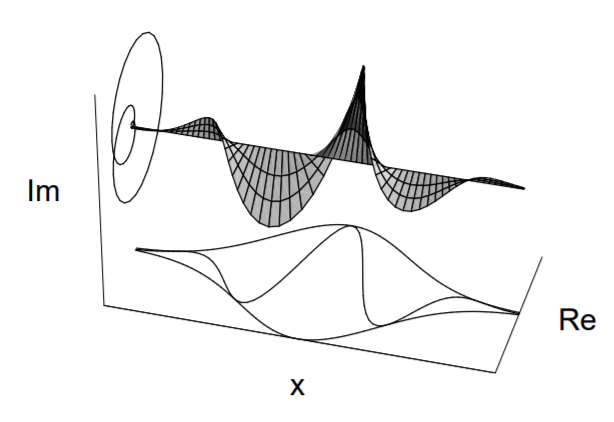
\includegraphics[scale=1]{1_19.PNG}
    \captionsetup{font={Large}}
    \caption{Gaussian wave package in the local area.}
    \label{fig:1.19}
\end{figure}
\\
\begin{equation}
\Psi(x, 0)=\frac{1}{\sqrt[4]{2 \pi \sigma}} e^{i k_{0} x} e^{-\left(x-x_{0}\right)^{2} / 4 \sigma}
\end{equation}\\
%公式 1.75
de ned. This form involves on the one hand the carrier $exp(ik_0x)$, on the other hand
the envelope end $exp[-(x-x_0)^2/4\sigma]$, as well as a normalization factor.
Even in $k$ space, the wavefunction has a Gaussian shape (and is therefore
normalizable for finite values ​​of $\sigma$),
\\
\begin{equation}
\begin{aligned} \Psi(k, 0) &=\mathcal{F}[\Psi(x, 0)]=\int d x \Psi(x, 0) e^{-i k x} \\ &=\sqrt[4]{8 \pi \sigma} e^{-i\left(k-k_{0}\right) x_{0}} e^{-\sigma\left(k-k_{0}\right)^{2}} \end{aligned}
\end{equation}\\
%公式 1.76
The propagation of a free massive particle is as usual via
the propagation of free plane waves with dispersion $E_k=\hbar^2 k^2/2m$,
\\
\begin{equation}
\begin{aligned} 
    \Psi(x, t) &=\int \frac{d k}{2 \pi} \Psi(k, 0) \exp \left[i\left(k x-\hbar k^{2} t / 2 m\right)\right] \\ 
    &=\sqrt[4]{8 \pi \sigma} \int \frac{d k}{2 \pi} e^{-i\left(k-k_{0}\right) x_{0}} e^{-\sigma\left(k-k_{0}\right)^{2}} e^{i\left(k x-\hbar k^{2} t / 2 m\right)}\\
    k \rightarrow & \underline{k+k_{0}} \sqrt[4]{8 \pi \sigma} e^{i k_{0} x} e^{-i \hbar k_{0}^{2} t / 2 m} \int \frac{d k}{2 \pi} e^{i k\left(x-\hbar k_{0} t / m-x_{0}\right)} e^{-i \hbar k^{2} t / 2 m} e^{-\sigma k^{2}} \\ 
    &=\sqrt[4]{\frac{\sigma}{2 \pi \sigma_{t}^{2}}} \underbrace{e^{i k_{0} x}} \underbrace{e^{i k_{0} x} e^{-i \hbar k_{0}^{2} t / 2 m}}_{\text {Phase }} e^{-\left(x-\hbar k_{0} t / m-x_{0}\right)^{2} / 4 \sigma_{t}} 
\end{aligned}
\end{equation}\\
%公式 1.77
%PAGE 43
with $\sigma_t=\sigma+i\hbar t/2m$. With the wave function (1.77) one finds the expectation values
\\
\begin{equation}
\begin{aligned}\langle x\rangle &= x_{0}+\frac{\hbar k_{0}}{m} t=x_{0}+v_{0} t \\\langle p\rangle &=\hbar\langle k\rangle=\hbar \int \frac{d k}{2 \pi} \Psi^{*}(k, 0) k \Psi(k, 0)=\hbar k_{0} \\(\Delta x)^{2} &=\left\langle\left(x-x_{0}-v_{0} t\right)^{2}\right\rangle= 2\left(\frac{1}{\sigma_{t}}+\frac{1}{\sigma_{t}^{*}}\right)^{-1}=\sigma\left(1+\frac{\hbar^{2} t^{2}}{4 m^{2} \sigma^{2}}\right) \\(\Delta p)^{2} &=\left\langle\left(p-\hbar k_{0}\right)^{2}\right\rangle=\frac{\hbar^{2}}{4 \sigma} \end{aligned}
\end{equation}\\
%公式 1.78
To determine $\triangle x^2$ we used a Gaussian distribution $\varpropto exp(-ax^2)$ has the width $\langle \triangle x^2 \rangle=1/2a$. With that we find the Zer
ow
of the wave packet linear in $t,\triangle x\varpropto t$, and the blur increases with time
to,
\\
\begin{equation}
\Delta x \Delta p=\frac{\hbar}{2} \sqrt{1+\frac{\hbar^{2} t^{2}}{4 m^{2} \sigma^{2}}} \geq \frac{\hbar}{2}
\end{equation}\\
%公式 1.79
Note that in Hamiltonian dynamics a packet is linear in time
cerium
If, $\triangle x\varpropto t$, the dissipative dynamics take a packet more slowly
cerium
asl, according to $\triangle x\varpropto \sqrt{t}$
\section{Location and momentum representation}
Let $f(\vec{r})\in \mathbb{C},\vec{r}\in\mathbb{R}^n$ given. The Fourier transformation
is a unit-is operation on the space of complex-valued functions.
Transferred to the space of the wave functions we get the representations
\\
\begin{equation}
\Psi(\vec{r}, t)=\int \frac{d^{n} p}{(2 \pi \hbar)^{n}} e^{i \vec{p} \cdot \vec{r} / \hbar} \Psi(\vec{p}, t)
\end{equation}\\
%公式 1.80
\\
\begin{equation}
\Psi(\vec{p}, t)=\int d^{n} r e^{-i \vec{p} \cdot \vec{r} / \hbar} \Psi(\vec{r}, t)
\end{equation}\\
%公式 1.81

%PAGE 44
\begin{equation}
\int d^{n} p e^{i \vec{p} \cdot \vec{r} / \hbar}=(2 \pi \hbar)^{n} \delta^{n}(\vec{r})
\end{equation}\\
%公式 1.82
interpretation
\{The plane wave $\phi_p=exp[i\vec{p}\cdot\vec{r}/\hbar]$, Eq. (1.57) describes a particle
with impulse $\vec{p}$. The impulse is sharp, according to the place unde -
($\phi_p$ can not be normalized, see later).
\{According to the superposition principle, (1.80) describes the function $\Psi(\vec{r},t)$
as superposition of partial waves $\phi_p$ with momentum $\vec{p}$.
From these two points one can conclude that $\Psi(\vec{p},t)$ the amplitude
of the particle at time t in the momentum space is the amplitude during $\Psi(\vec{x},t)$
of the particle in space).
It is
\\
\begin{equation}
|\Psi(\vec{r}, t)|^{2} d^{n} r
\end{equation}\\
%公式 1.83
the probability of the particle at time $t$ in volume $d^nr$ to $\vec{r}$
and analogously one interprets
\\
\begin{equation}
|\Psi(\vec{p}, t)|^{2} \frac{d^{n} p}{(2 \pi \hbar)^{n}}
\end{equation}\\
%公式 1.84
as the probability that the particle at time t the momentum in $d^np$
around \~{} p. We call
\\
\begin{equation}
\begin{array}{l}{\Psi(\vec{r}, t): \text { the wave function in spatial representation, }} \\ {\Psi(\vec{p}, t): \text { the wave function in pulse representation. }}\end{array}
\end{equation}\\
%公式 1.85
The Fourier transformation transforms between position and momentum representation,
the standardization is preserved,
\\
\begin{equation}
\int d^{n} r|\Psi(\vec{r}, t)|^{2} \quad \stackrel{\text { Parseval }}{=} \int \frac{d^{n} p}{(2 \pi \hbar)^{n}}|\Psi(\vec{p}, t)|^{2}
\end{equation}\\
%公式 1.86
Between these two representations a basic transformation--
We will discuss this in detail in the next chapter. At this point
Let us mention the different bases (location and momentum base with sharp
Location $\vec{r_0}$ and momentum $\vec{p}_0$) in the location (O-Dar) and momentum representations
(I-Dar) (note that these expressions are distributive or not normalizable):
\\
\begin{equation}
\begin{array}{ll}{\text { local base in O-Dar }} & {\Psi_{\vec{r}_{0}}(\vec{r})=\delta^{n}\left(\vec{r}-\vec{r}_{0}\right)} \\ {\text { pulse base in I-Dar }} & {\Psi_{\vec{p}_{0}}(\vec{p})=(2 \pi \hbar)^{n} \delta^{n}\left(\vec{p}-\vec{p}_{0}\right)}\end{array}
\end{equation}\\
%公式 1.87

%PAGE 45
\begin{equation}
\begin{array}{ll}{\text { Ipulse base in O-Dar }} & {\Psi_{\vec{p}_{0}}(\vec{r})=\int \frac{d^{n} p}{(2 \pi \hbar)^{n}} \Psi_{\vec{p}_{0}}(\vec{p}) e^{i \vec{p} \cdot \vec{r} / \hbar}=e^{i \vec{p}_{0} \cdot \vec{r} / \hbar}} \\ {\text { local base in } \mathrm{I}_{-} \mathrm{Dar}} & {\Psi_{\vec{r}_{0}}(\vec{p})=\int d^{n} r \Psi_{\vec{r}_{0}}(\vec{r}) e^{-i \vec{p} \cdot \vec{r} / \hbar}=e^{-i \vec{p} \cdot \vec{r}_{0} / \hbar}}\end{array}
\end{equation}\\
%
%公式 1.88
\newpage